\documentclass[dvipsnames, svgnames, x11names, a4paper, 11pt]{article}

% URLs and hyperlinks ------------------------------
\usepackage{hyperref}
\hypersetup{
    colorlinks=true,
    linkcolor=NavyBlue,
    filecolor=magenta,      
    urlcolor=blue,
}
\usepackage{xurl}
%---------------------------------------------------

\usepackage{adjustbox}
\usepackage{float}
\usepackage{graphicx}
\usepackage{listings}
\usepackage{color}
\usepackage{xcolor}
\usepackage{subfigure}

\definecolor{dkgreen}{rgb}{0,0.6,0}
\definecolor{gray}{rgb}{0.5,0.5,0.5}
\definecolor{mauve}{rgb}{0.58,0,0.82}

\lstset{frame=tb,
    language=vhdl,
    aboveskip=3mm,
    belowskip=3mm,
    showstringspaces=false,
    columns=flexible,
    basicstyle=\ttfamily,
    numbers=left,
    numberstyle=\small\color{gray},
    keywordstyle=\bfseries\color{Green4},
    commentstyle=\color{gray},
    stringstyle=\color{mauve},
    breaklines=true,
    breakatwhitespace=true,
    tabsize=4,
    identifierstyle=\color{black}
}

\usepackage{tikz}
\usetikzlibrary{automata, positioning, arrows}

\usepackage{xepersian}
\settextfont{Yas}

\title{تمرین چراغ راهنمایی و رانندگی}
\author{
فاطمه علی‌ملکی \\
مهدی حق‌وردی
}
\begin{document}
\maketitle
\tableofcontents
\newpage

\section{دیاگرام}\label{digram}
\begin{latin}
\begin{figure}[ht]
\begin{center}
\begin{adjustbox}{width=\textwidth}
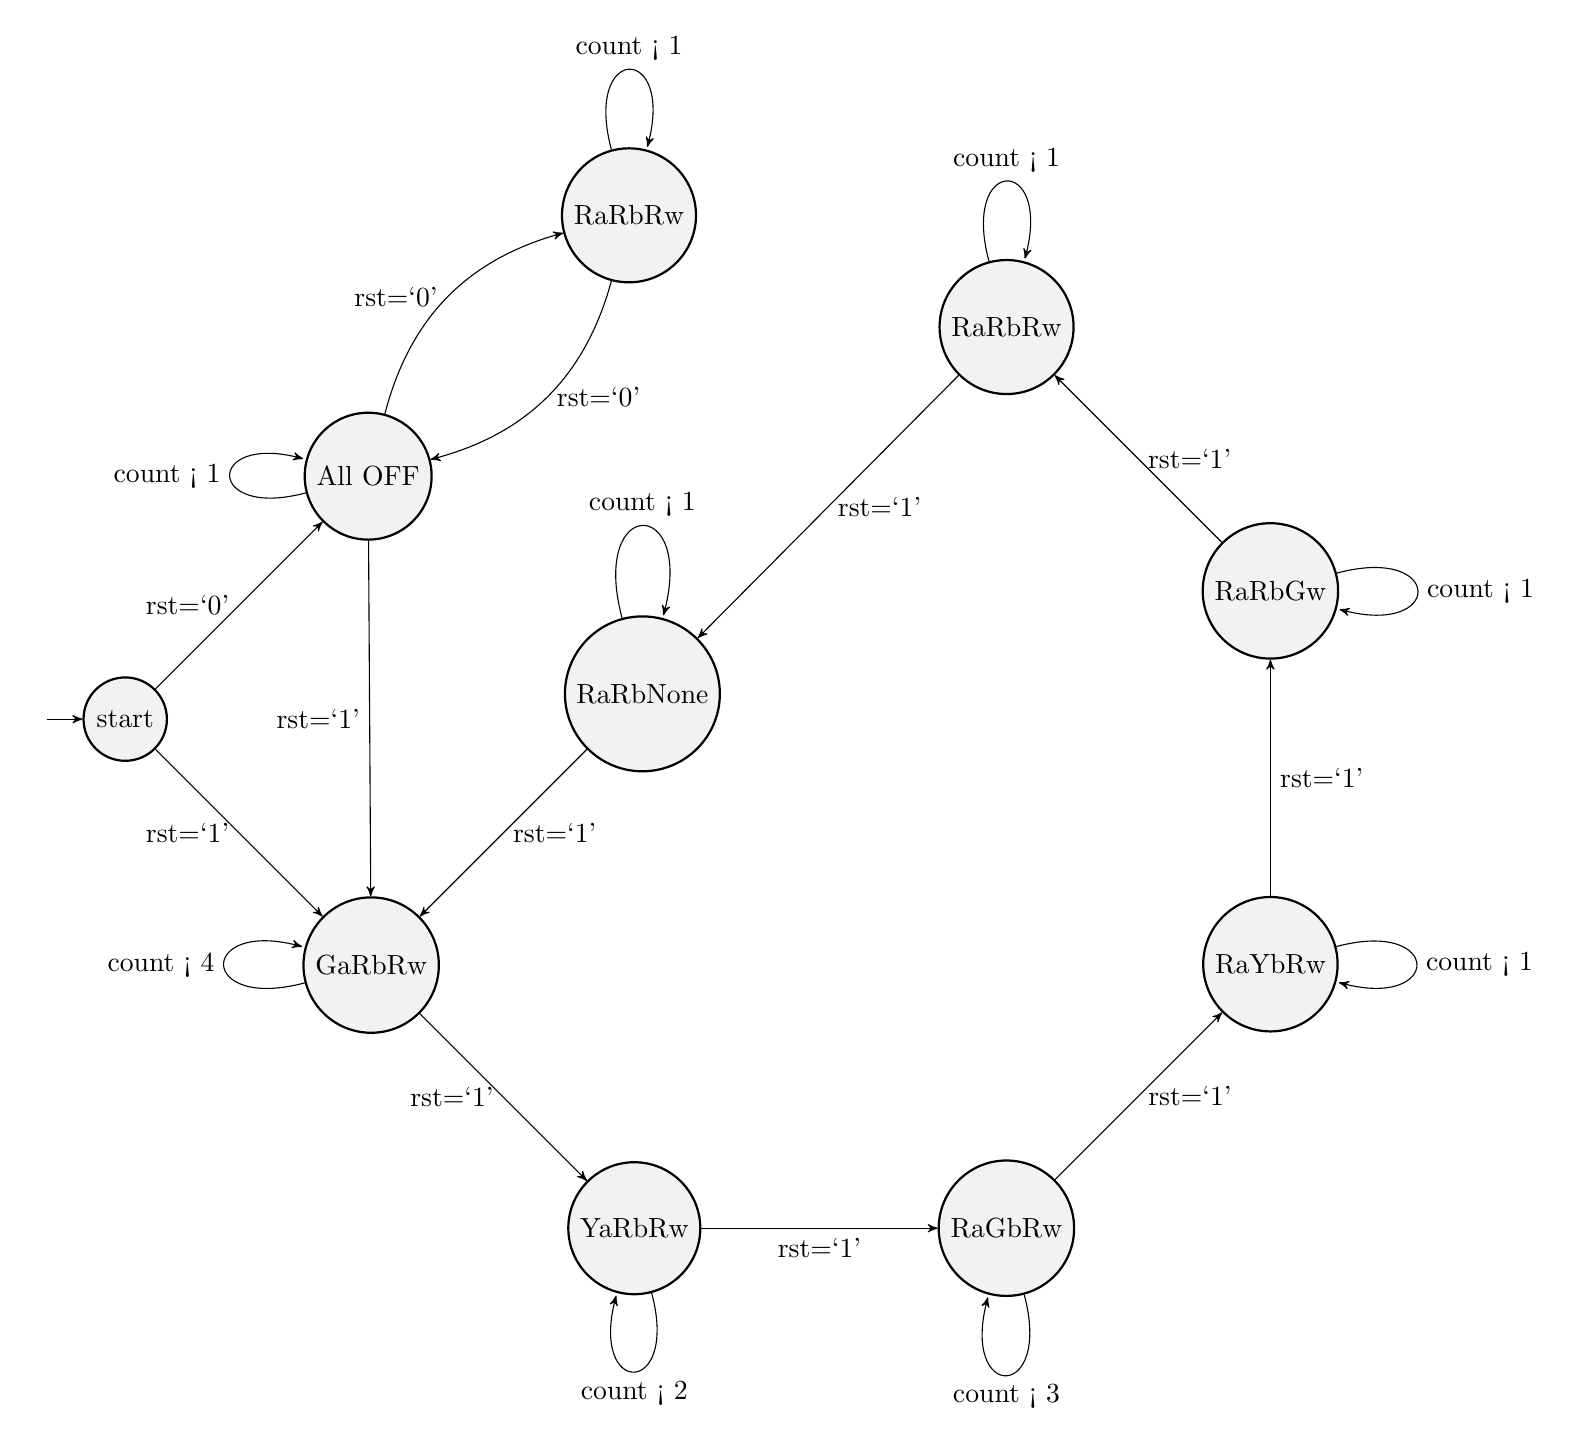
\begin{tikzpicture}
[->,
 >=stealth',
 node distance=3cm,
 every state/.style={thick,fill=gray!10,
 initial text=$$},
]


\node[state, initial]     (start) {start};
\node[state, below right=of start] (s0) {GaRbRw};
\node[state, below right=of s0] (s1) {YaRbRw};
\node[state, right=of s1] (s2) {RaGbRw};
\node[state, above right=of s2] (s3) {RaYbRw};
\node[state, above=of s3] (s4) {RaRbGw};
\node[state, above right=of start] (s6) {All OFF};
\node[state, above right=of s6] (s5) {RaRbRw};
\node[state, above left=of s4] (s51) {RaRbRw};
\node[state, above right=of s0] (s7) {RaRbNone};


\draw
(start)    edge[left, left]   node{rst=`0'} (s6)
(start)    edge[right, left]   node{rst=`1'} (s0)

(s6)  edge[bend left, left]   node{rst=`0'} (s5)
(s5)  edge[bend left, right]   node{rst=`0'} (s6)

(s0)  edge[right, left]  node{rst=`1'} (s1)
(s1)  edge[right, below]  node{rst=`1'} (s2)
(s2)  edge[right, right]  node{rst=`1'} (s3)
(s3)  edge[below, right]  node{rst=`1'} (s4)
(s4)  edge[right, right]  node{rst=`1'} (s51)
(s51)  edge[right, right]  node{rst=`1'} (s7)
(s7)  edge[right, right]  node{rst=`1'} (s0)
(s6)  edge[left]  node{rst=`1'} (s0)

(s0)   edge[loop left]          node{count < 4} (s0)
(s1)   edge[loop below]         node{count < 2} (s1)
(s2)   edge[loop below]         node{count < 3} (s2)
(s3)   edge[loop right]         node{count < 1} (s3)
(s4)   edge[loop right]         node{count < 1} (s4)
(s5)   edge[loop above]         node{count < 1} (s5)
(s51)   edge[loop above]         node{count < 1} (s51)
(s7)   edge[loop above]         node{count < 1} (s7)
(s6)   edge[loop left]         node{count < 1} (s6);
\end{tikzpicture}
\end{adjustbox}
\end{center}
\end{figure}
\end{latin}

در این دیاگرام، وضعیت‌های ماشین کشیده شده‌اند. یال‌های حلقه روی وضعیت‌ها میزان زمان ایستادن روی آن وضعیت هستند.

\section{توضیحات}
در این قسمت توضیحاتی راجع به کد‌ها می‌دهیم.

\subsection{\lr{\texttt{clock\_divide.vhdl}}}
که قبلا توضیح داده شده و تعداد کلاک 
\lr{100 MHz}
را به عدد
\lr{1 MHz}
تبدیل می‌کند.
\newpage
\subsection{\lr{\texttt{trfc.ucf}}}
با مراجعه به توضیحات سایت تولید کننده‌ی برد این فایل را نوشتیم.
\begin{figure}[H]
\begin{center}
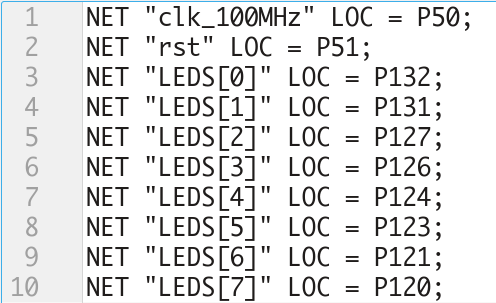
\includegraphics[width=0.5\textwidth, height=0.23\textheight]{./images/ucf}
\end{center}
\end{figure}

\subsection{\lr{\texttt{traffic.vhdl}}}
\subsubsection{موجودیت \lr{\texttt{traffic}}}
\begin{latin}
\begin{lstlisting}
library IEEE;
use IEEE.STD_LOGIC_1164.all;
use IEEE.STD_LOGIC_unsigned.all;

entity traffic is
    port (
        clk_100MHZ: in std_logic;
        rst: in std_logic;
        LEDS: out std_logic_vector(7 downto 0)
    );
end traffic;
\end{lstlisting}
\end{latin}
\begin{itemize}
\item \lr{\texttt{clk\_100MHZ}}:
کلاک ورودی از برد.

\item \lr{\texttt{rst}}:
دکمه‌ی \lr{K1}

\item \lr{\texttt{LEDS}}:
چراغ‌های \lr{LED}
\end{itemize}
\newpage

\subsubsection{معماری}
\begin{latin}
\begin{lstlisting}[firstnumber=12]
architecture traffic of traffic is
    component clock_divide
        port (
            clk_in: in std_logic;
            clk_out: out std_logic
        );
	end component;

    -- clock
    signal clk_1Hz: std_logic;

    -- states
    type state_type is (s0, s1, s2, s3, s4, s5, s6, s7);
    signal state: state_type;

    -- state counter
    signal count: std_logic_vector(2 downto 0);

begin
clock_divider: clock_divide port map (clk_100MHZ, clk_1Hz);
\end{lstlisting}
\end{latin}
ابتدا
از موجودیت 
\lr{\texttt{clock\_divider}}
یک کامپوننت تعریف می‌کنیم تا بتوانیم از آن استفاده کنیم، سپس ۳ سیگنال تعریف می‌کنیم:
\begin{itemize}
\item \lr{\texttt{clk\_1Hz}}

این سیگنال، مقدار خروجی کامپوننت 
\lr{\texttt{clock\_divider}}
را دریافت می‌کند.

\item \lr{\texttt{state}}

این سیگنال از نوع 
\lr{\texttt{state\_type}}
است که بالای سیگنال تعریف شده و مقادیر 
\lr{state}های
موجود در دیاگرام (\ref{digram}) را می‌تواند داشته باشد.

\item \lr{\texttt{count}}

سیگنالی برای شماره ثانیه‌ها؛ به کمک این سیگنال بین 
\lr{state}ها
جابجا می‌شویم.
\end{itemize}

\newpage
\subsubsection{اولین فرآیند}
\begin{latin}
\begin{lstlisting}[firstnumber=29]
process(clk_1Hz, rst)
-- needed variables
variable one_sec   : std_logic_vector(2 downto 0) := '001';
variable two_sec   : std_logic_vector(2 downto 0) := '010';
variable three_sec : std_logic_vector(2 downto 0) := '011';
variable four_sec  : std_logic_vector(2 downto 0) := '100';

begin
	if rst = '1' then
        if clk_1Hz'event and clk_1Hz = '1' then
            case state is
                when s0 =>
                    if count < four_sec then
                        state <= s0;
                        count <= count + 1;
                    else
                        state <= s1;
                        count <= "000";
                    end if;
                when s1 =>
                    if count < two_sec then
                        state <= s1;
                        count <= count + 1;
                    else
                        state <= s2;
                        count <= "000";
                    end if;
                when s2 =>
                    if count < three_sec then
                        state <= s2;
                        count <= count + 1;
                    else
                        state <= s3;
                        count <= "000";
                    end if;
                when s3 =>
                    if count < one_sec then
                        state <= s3;
                        count <= count + 1;
                    else
                        state <= s4;
                        count <= "000";
                    end if;
                when s4 =>
                    if count < two_sec then
                        state <= s4;
                        count <= count + 1;
                    else
                        state <= s5;
                        count <= "000";
                    end if;
                when s5 =>
                    if count < one_sec then
                        state <= s5;
                        count <= count + 1;
                    else
                        state <= s7;
                        count <= "000";
                    end if;
                when s7 =>
                    if count < one_sec then
                        state <= s7;
                        count <= count + 1;
                    else
                        state <= s0;
                        count <= "000";
                    end if;
                when others =>
                    state <= s0;
                    count <= "000";
            end case;
        end if;
\end{lstlisting}
\end{latin}

این فرآیند، به کلاک ۱ هرتز و کلید \lr{\texttt{rst}} حساس است. سپس به اندازه‌ی مقدار ثانیه‌هایی که در فایل پروژه نوشته شده است، متغیر‌هایی تعریف می‌کنیم تا از آنها استفاده کنیم.

این فرآیند یک بلاک \lr{\texttt{if}} بزرگ دارد که از بین ۰ و ۱ (مقادیر \lr{\texttt{rst}}) انتخاب می‌کند؛ اگر مقدار آن ۱ باشد، وارد حلقه‌ی بزرگ‌‌تر دیاگرام (\ref{digram}) می‌شویم.

از بین 
\lr{state}های
\lr{s0}
تا
\lr{s6}
با توجه به زمانی که برای هر کدام تعریف شده، چرخش انجام می‌دهیم.

این فرآیند، وقتی که مقدار 
\lr{\texttt{state}}
را تغییر می‌دهد، فرآیند دیگر را (\ref{second-process}) بیدار می‌کند که در ادامه به توضیح آن می‌پردازیم.

\newpage
\subsubsection{قسمت \lr{\texttt{else}}}
\begin{latin}
\begin{lstlisting}[firstnumber=101]
    else  -- rst = '0'
        if clk_1Hz'event and clk_1Hz = '1' then
			if state /= s5 and state /= s6 then
				state <= s5;
				count <= "000";
			end if;
			case state is
				when s5 =>
					if count < one_sec then
						state <= s5;
						count <= count + 1;
					else
						state <= s6;
						count <= "000";
					end if;
				when s6 =>
					if count < one_sec then
						state <= s6;
						count <= count + 1;
					else
						state <= s5;
						count <= "000";
					end if;
				when others =>
					state <= s5;
					count <= "000";
            end case;
        end if;
    end if;
end process;
\end{lstlisting}
\end{latin}

در این قسمت، اگر مقدار \lr{\texttt{rst}} صفر باشد، ابتدا چک می‌کنیم که آیا در 
\lr{state}
۵\RTLfootnote{\lr{RaRbRw}}
 یا ۶\RTLfootnote{\lr{All OFF}} نیستیم به 
\lr{state}
۵ برویم. سپس با توجه به دیاگرام، بین این دو 
\lr{state}
می‌چرخیم، تا رفتار خواسته شده نمایش داده شود.

\newpage
\subsubsection{فرآیند دوم}
\label{second-process}
\begin{latin}
\begin{lstlisting}[firstnumber=131]
process(state)
begin
case state is
		-- Red Yellow Green, Red Yellow Green, Red Green
		when s0 => LEDS <= "00110010"; -- Ga=1, Rb=1, Rw=1
		when s1 => LEDS <= "01010010"; -- Ya=1, Rb=1, Rw =1
		when s2 => LEDS <= "10000110"; -- Ra=1, Gb=1, Rw=1
		when s3 => LEDS <= "10001010"; -- Ra=1, Yb=1, Rw=1
		when s4 => LEDS <= "10010001"; -- Ra=1, Rb=1, Gw=1
		when s5 => LEDS <= "10010010"; -- Ra=1, Rb=1, Rw=1
		when s6 => LEDS <= "00000000"; -- All LEDs are off
        when s7 => LEDS <= "10010000"; -- Ra=1, Rb=1, Rw=0
		when others => LEDS <= "00110010"; -- Ga=1, Rb=1, Rw=1
end case;
end process;
end traffic;
\end{lstlisting}
\end{latin}

این فرآیند، به مقدار 
\lr{\texttt{state}}
حساس است و با توجه به مقدار 
\lr{\texttt{state}}
چراغ‌های لازم را روشن می‌کند.
\end{document}
